% Options for packages loaded elsewhere
\PassOptionsToPackage{unicode}{hyperref}
\PassOptionsToPackage{hyphens}{url}
\PassOptionsToPackage{dvipsnames,svgnames,x11names}{xcolor}
%
\documentclass[
  letterpaper,
  DIV=11,
  numbers=noendperiod]{scrartcl}

\usepackage{amsmath,amssymb}
\usepackage{iftex}
\ifPDFTeX
  \usepackage[T1]{fontenc}
  \usepackage[utf8]{inputenc}
  \usepackage{textcomp} % provide euro and other symbols
\else % if luatex or xetex
  \usepackage{unicode-math}
  \defaultfontfeatures{Scale=MatchLowercase}
  \defaultfontfeatures[\rmfamily]{Ligatures=TeX,Scale=1}
\fi
\usepackage{lmodern}
\ifPDFTeX\else  
    % xetex/luatex font selection
    \setmonofont[Scale=0.5]{Latin Modern Mono}
\fi
% Use upquote if available, for straight quotes in verbatim environments
\IfFileExists{upquote.sty}{\usepackage{upquote}}{}
\IfFileExists{microtype.sty}{% use microtype if available
  \usepackage[]{microtype}
  \UseMicrotypeSet[protrusion]{basicmath} % disable protrusion for tt fonts
}{}
\makeatletter
\@ifundefined{KOMAClassName}{% if non-KOMA class
  \IfFileExists{parskip.sty}{%
    \usepackage{parskip}
  }{% else
    \setlength{\parindent}{0pt}
    \setlength{\parskip}{6pt plus 2pt minus 1pt}}
}{% if KOMA class
  \KOMAoptions{parskip=half}}
\makeatother
\usepackage{xcolor}
\usepackage[top=20mm,left=20mm,bottom=20mm,right=20mm]{geometry}
\setlength{\emergencystretch}{3em} % prevent overfull lines
\setcounter{secnumdepth}{5}
% Make \paragraph and \subparagraph free-standing
\makeatletter
\ifx\paragraph\undefined\else
  \let\oldparagraph\paragraph
  \renewcommand{\paragraph}{
    \@ifstar
      \xxxParagraphStar
      \xxxParagraphNoStar
  }
  \newcommand{\xxxParagraphStar}[1]{\oldparagraph*{#1}\mbox{}}
  \newcommand{\xxxParagraphNoStar}[1]{\oldparagraph{#1}\mbox{}}
\fi
\ifx\subparagraph\undefined\else
  \let\oldsubparagraph\subparagraph
  \renewcommand{\subparagraph}{
    \@ifstar
      \xxxSubParagraphStar
      \xxxSubParagraphNoStar
  }
  \newcommand{\xxxSubParagraphStar}[1]{\oldsubparagraph*{#1}\mbox{}}
  \newcommand{\xxxSubParagraphNoStar}[1]{\oldsubparagraph{#1}\mbox{}}
\fi
\makeatother


\providecommand{\tightlist}{%
  \setlength{\itemsep}{0pt}\setlength{\parskip}{0pt}}\usepackage{longtable,booktabs,array}
\usepackage{calc} % for calculating minipage widths
% Correct order of tables after \paragraph or \subparagraph
\usepackage{etoolbox}
\makeatletter
\patchcmd\longtable{\par}{\if@noskipsec\mbox{}\fi\par}{}{}
\makeatother
% Allow footnotes in longtable head/foot
\IfFileExists{footnotehyper.sty}{\usepackage{footnotehyper}}{\usepackage{footnote}}
\makesavenoteenv{longtable}
\usepackage{graphicx}
\makeatletter
\def\maxwidth{\ifdim\Gin@nat@width>\linewidth\linewidth\else\Gin@nat@width\fi}
\def\maxheight{\ifdim\Gin@nat@height>\textheight\textheight\else\Gin@nat@height\fi}
\makeatother
% Scale images if necessary, so that they will not overflow the page
% margins by default, and it is still possible to overwrite the defaults
% using explicit options in \includegraphics[width, height, ...]{}
\setkeys{Gin}{width=\maxwidth,height=\maxheight,keepaspectratio}
% Set default figure placement to htbp
\makeatletter
\def\fps@figure{htbp}
\makeatother

\KOMAoption{captions}{tableheading}
\makeatletter
\@ifpackageloaded{tcolorbox}{}{\usepackage[skins,breakable]{tcolorbox}}
\@ifpackageloaded{fontawesome5}{}{\usepackage{fontawesome5}}
\definecolor{quarto-callout-color}{HTML}{909090}
\definecolor{quarto-callout-note-color}{HTML}{0758E5}
\definecolor{quarto-callout-important-color}{HTML}{CC1914}
\definecolor{quarto-callout-warning-color}{HTML}{EB9113}
\definecolor{quarto-callout-tip-color}{HTML}{00A047}
\definecolor{quarto-callout-caution-color}{HTML}{FC5300}
\definecolor{quarto-callout-color-frame}{HTML}{acacac}
\definecolor{quarto-callout-note-color-frame}{HTML}{4582ec}
\definecolor{quarto-callout-important-color-frame}{HTML}{d9534f}
\definecolor{quarto-callout-warning-color-frame}{HTML}{f0ad4e}
\definecolor{quarto-callout-tip-color-frame}{HTML}{02b875}
\definecolor{quarto-callout-caution-color-frame}{HTML}{fd7e14}
\makeatother
\makeatletter
\@ifpackageloaded{caption}{}{\usepackage{caption}}
\AtBeginDocument{%
\ifdefined\contentsname
  \renewcommand*\contentsname{Table of contents}
\else
  \newcommand\contentsname{Table of contents}
\fi
\ifdefined\listfigurename
  \renewcommand*\listfigurename{List of Figures}
\else
  \newcommand\listfigurename{List of Figures}
\fi
\ifdefined\listtablename
  \renewcommand*\listtablename{List of Tables}
\else
  \newcommand\listtablename{List of Tables}
\fi
\ifdefined\figurename
  \renewcommand*\figurename{Figure}
\else
  \newcommand\figurename{Figure}
\fi
\ifdefined\tablename
  \renewcommand*\tablename{Table}
\else
  \newcommand\tablename{Table}
\fi
}
\@ifpackageloaded{float}{}{\usepackage{float}}
\floatstyle{ruled}
\@ifundefined{c@chapter}{\newfloat{codelisting}{h}{lop}}{\newfloat{codelisting}{h}{lop}[chapter]}
\floatname{codelisting}{Listing}
\newcommand*\listoflistings{\listof{codelisting}{List of Listings}}
\makeatother
\makeatletter
\makeatother
\makeatletter
\@ifpackageloaded{caption}{}{\usepackage{caption}}
\@ifpackageloaded{subcaption}{}{\usepackage{subcaption}}
\makeatother

\ifLuaTeX
  \usepackage{selnolig}  % disable illegal ligatures
\fi
\usepackage{bookmark}

\IfFileExists{xurl.sty}{\usepackage{xurl}}{} % add URL line breaks if available
\urlstyle{same} % disable monospaced font for URLs
\hypersetup{
  pdftitle={How do trees grow in Western North America:A new modeling approach},
  colorlinks=true,
  linkcolor={blue},
  filecolor={Maroon},
  citecolor={Blue},
  urlcolor={Blue},
  pdfcreator={LaTeX via pandoc}}


\title{How do trees grow in Western North America:\newline A new
modeling approach}
\author{}
\date{}

\begin{document}
\maketitle


\section{The motivations behind the
project}\label{the-motivations-behind-the-project}

\begin{tcolorbox}[enhanced jigsaw, breakable, arc=.35mm, colframe=quarto-callout-tip-color-frame, bottomrule=.15mm, colbacktitle=quarto-callout-tip-color!10!white, leftrule=.75mm, opacityback=0, opacitybacktitle=0.6, toptitle=1mm, colback=white, bottomtitle=1mm, titlerule=0mm, toprule=.15mm, rightrule=.15mm, left=2mm, title=\textcolor{quarto-callout-tip-color}{\faLightbulb}\hspace{0.5em}{The technical motivation}, coltitle=black]

Bayesian magic! We fit all together the low frequency, decadal (to
centennial) variations (the \emph{detrending}) \textbf{and} the climatic
variations (of interest). We let the model and the data speak,
i.e.~disentangle allometry (age/size trends in growth) from climate.
This way, we avoid many arbitrary modeling decision (e.g.~when one has
to choose the frequency cut-off of a spline). And all the uncertainties
get propagated to any decisions/predictions.

\end{tcolorbox}

\hfill\break

\begin{tcolorbox}[enhanced jigsaw, breakable, arc=.35mm, colframe=quarto-callout-tip-color-frame, bottomrule=.15mm, colbacktitle=quarto-callout-tip-color!10!white, leftrule=.75mm, opacityback=0, opacitybacktitle=0.6, toptitle=1mm, colback=white, bottomtitle=1mm, titlerule=0mm, toprule=.15mm, rightrule=.15mm, left=2mm, title=\textcolor{quarto-callout-tip-color}{\faLightbulb}\hspace{0.5em}{The ecological motivation}, coltitle=black]

Tree ring data offers offer an unique opportunity to learn how trees
grow in a changing climate, through the complex interactions between
external events and size-dependent developmental stages. While
dendrochronology has mostly focus on past climate reconstructions, our
approach do not try to standardize away the complexities of
individual-level growth and species-specific variations. On the
contrary, we believe that this complexity---if handle correctly by a
model---can help us understand how tree growth varies within and
\textbf{across species, ecosystems, and climates}. And \emph{in fine}
our approach could improve our forecasts of forest dynamics, carbon
sequestration, and thus climate change itself!

\end{tcolorbox}

\section{A quick summary of the
model}\label{a-quick-summary-of-the-model}

Before diving into the results of our first inferences, let's describe
the model!\\
We can divide the model in two main parts:

\begin{itemize}
\item
  the mid- to long-term processes that are not directly related to
  climate, \newline such as \textbf{allometric constraints}, neighbour
  competition dynamics, \ldots{}
\item
  the short-term variations that are related to external conditions,
  \newline mostly \textbf{climate}, but also pest outbreaks, \ldots{}
\end{itemize}

\subsection{Mid- to long-term
processes}\label{mid--to-long-term-processes}

When we think about these low frequency variations, we mainly think
about the age/size trends that affect tree growth, due to the natural
size and shape of trees. We want this part of the model to be
\textbf{flexible} enough to accommodates phase shifts, since tree growth
is rarely perfectly smooth.\\

\begin{center}
\includegraphics{summary_currentprogress_files/figure-pdf/unnamed-chunk-3-1.pdf}
\end{center}

We believe that these variations are ``\emph{not directly related to
climate}'', but not totally independent of the climate neither: a big
storm could knock down surrounding trees and reduce competition for an
individual.

We model these variations with a first \textbf{Gaussian process} (GP).
The GP is characterized by a covariance function that captures the
temporal correlation between ring widths that persists over one or
several decades. The \textbf{length scale} \(\mathbf{\rho}\) of this
covariance function determined how quickly the correlations between ring
widths decay. In the example below, ring width \(x_2\) is more related
to \(x_1\) than \(x_3\) is.\\

\begin{center}
\includegraphics{summary_currentprogress_files/figure-pdf/unnamed-chunk-4-1.pdf}
\end{center}

The correlation across ring widths becomes negligeable around \(3\rho\)
years. \newpage

This mid- to long-term GP allows to capture, at the individual tree
level, the low frequency variations that appear in the ring width
measurements.\\

\begin{center}
\includegraphics{summary_currentprogress_files/figure-pdf/unnamed-chunk-5-1.pdf}
\end{center}

Since we expect some difference across fast- or slow-growing species, we
allow the length scale parameter to \textbf{vary across species}.

\subsection{Short-term variations}\label{short-term-variations}

When we think about these low frequency variations, we mainly think
about the yearly climatic conditions that explain short-term variations
in growth. We first believed that these climatic effects were shared
across conspecific trees within the same stand---in other words, that
the trees from the same species on the same stand would have the same
decrease/increase in growth because they experience similar climatic
conditions. But we will see that it's a bit more complex than!

\subsubsection{Climatic predictors
(stand-level)}\label{climatic-predictors-stand-level}

This part of the model is quite simple.\\
We selected three climatic predictors that are believed to have a strong
impact on tree growth:

\begin{itemize}
\tightlist
\item
  growing degree days (GDD, between )\\
\item
  soil moisture (SM, ) -- which is mostly driven by winter
  precipitation\\
\item
  vapor pressure deficit (VPD, )
\end{itemize}

\begin{tcolorbox}[enhanced jigsaw, breakable, arc=.35mm, colframe=quarto-callout-note-color-frame, bottomrule=.15mm, colbacktitle=quarto-callout-note-color!10!white, leftrule=.75mm, opacityback=0, opacitybacktitle=0.6, toptitle=1mm, colback=white, bottomtitle=1mm, titlerule=0mm, toprule=.15mm, rightrule=.15mm, left=2mm, title=\textcolor{quarto-callout-note-color}{\faInfo}\hspace{0.5em}{Note}, coltitle=black]

We extracted climate from \texttt{WLDAS}, which is available from 1980,
at a X-m resolution.\\
Since we plan to run our model from 1900 onward, we will also use
\texttt{PRISM} (with simpler predictors, likely GDD and winter
precipitation only).

\end{tcolorbox}

These 3 predictors are combined within a simple linear regression. We
allow the effect of each predictor to \textbf{vary across species}
(i.e.~we estimate species-specific slopes \(\beta\)).\\
This allows to identify different sensitivities between species, and
differentiate between Gymnosperms (in blue) and Angiosperms (in green).

\begin{center}
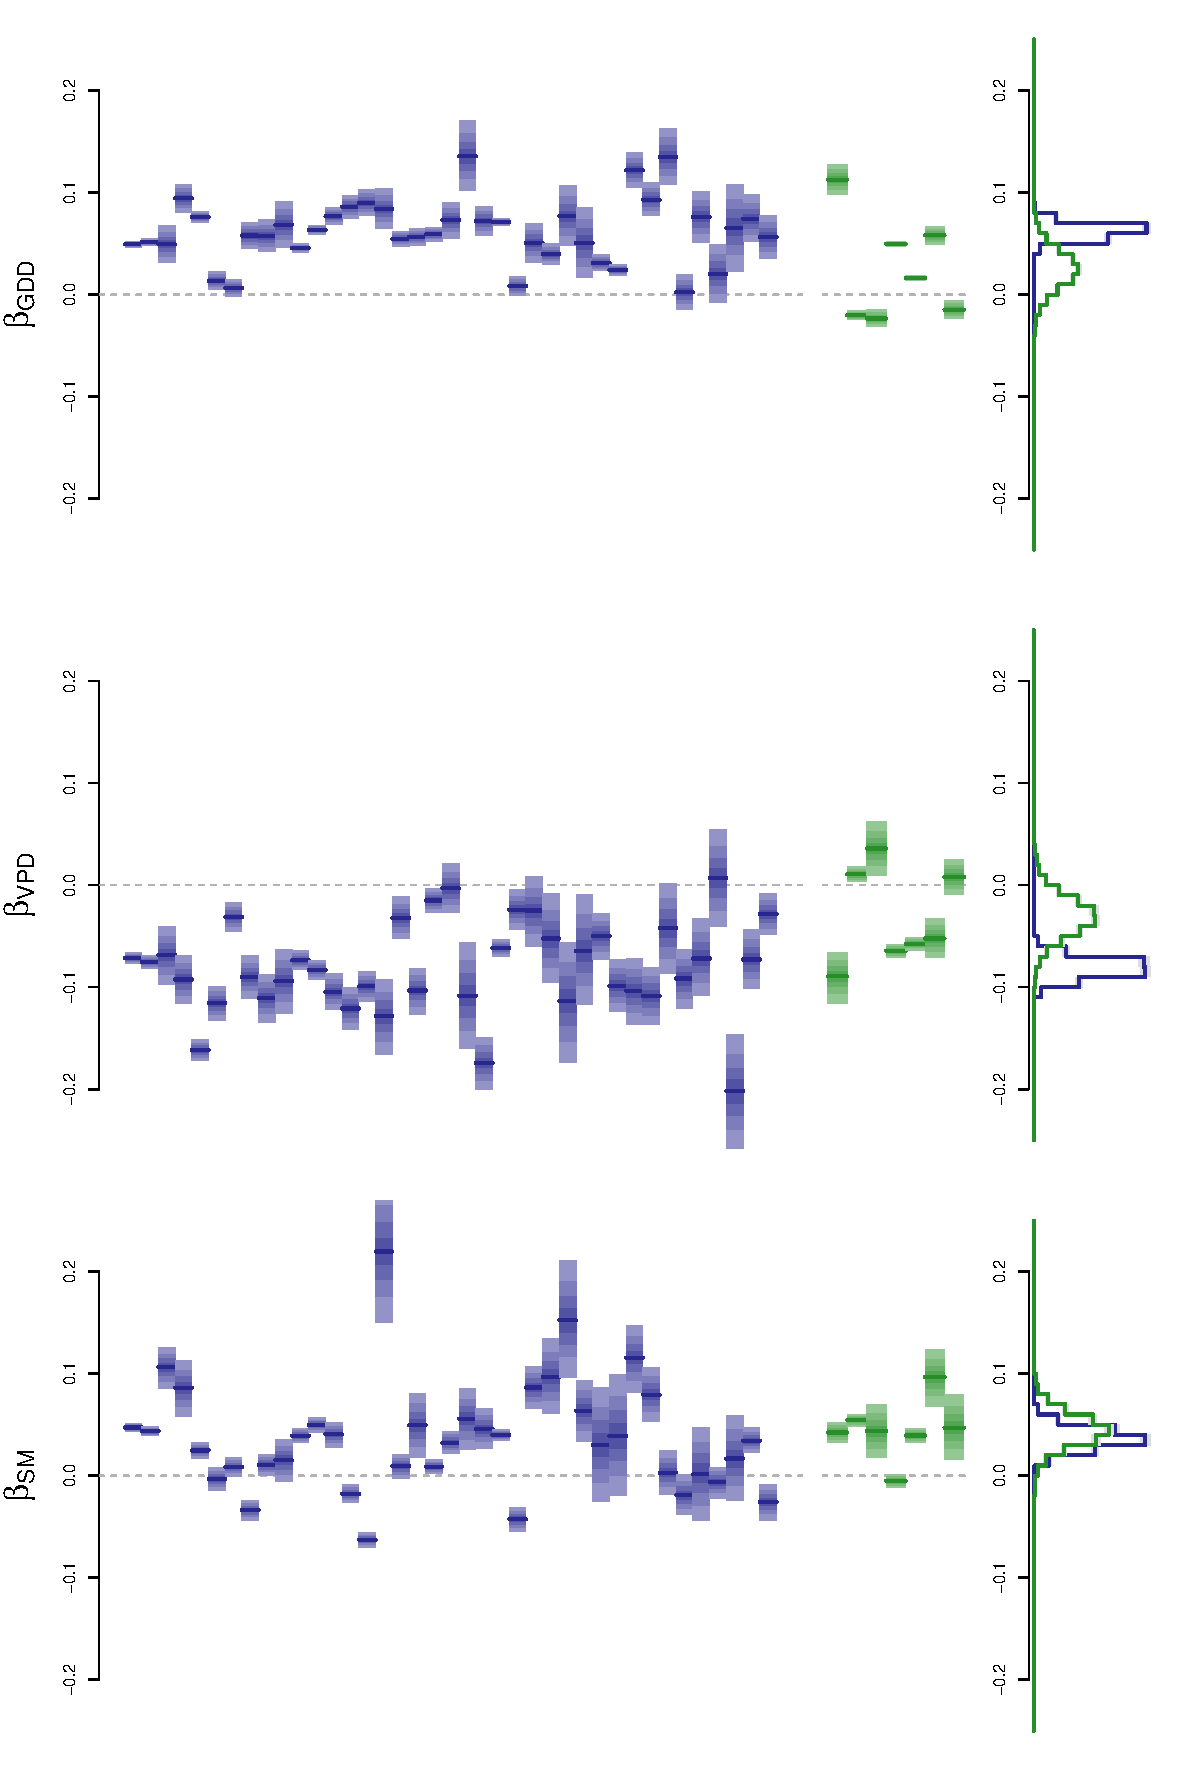
\includegraphics[width=0.7\textwidth,height=\textheight]{../../../analysis/pnwandmore/figures/newyork2025/model_estimates/climate_slopes_posterior_distributions.pdf}
\end{center}

In the left panel of this figure, each bar represents the posterior
distribution of a species-specific slope. The right part shows the
clade-level estimate (i.e.~Gymnosperms or Angiosperms).

\subsubsection{Shared residual variations
(stand-level)}\label{shared-residual-variations-stand-level}

The above predictors are not sufficient to capture the \textbf{shared
variations} of growth across trees within the same stand.\\
We added a short-term GP, initially with the goal to capture 3 to 5-year
patterns. But the model consistently finds some yearly residual
variation. In other words, the length scale of this GP is consistently
around 1 year.

\begin{tcolorbox}[enhanced jigsaw, breakable, arc=.35mm, colframe=quarto-callout-note-color-frame, bottomrule=.15mm, colbacktitle=quarto-callout-note-color!10!white, leftrule=.75mm, opacityback=0, opacitybacktitle=0.6, toptitle=1mm, colback=white, bottomtitle=1mm, titlerule=0mm, toprule=.15mm, rightrule=.15mm, left=2mm, title=\textcolor{quarto-callout-note-color}{\faInfo}\hspace{0.5em}{Note}, coltitle=black]

While the long-term GP was at the individual level (each tree gets its
own individual GP, determined by a species-specific length scale), this
short-term GP is shared across all trees in the same stand -- and we
estimate only one length scale across all stands.

\end{tcolorbox}

\subsubsection{Shocks!}\label{shocks}

Show that it's on drought years, but some other years are similarly dry.




\end{document}
